\section{Ontwerp}
Voor dit onderzoek heb ik een virtuele omgeving ontworpen met meer dan 48m$^2$
aan bewandelbare ruimte, de proefpersoon kan deze omgeving volledig verkennen en
toch in een 3 m x 4 m tracking area blijven. Deze virtuele omgeving bestaat uit 
een lange gang met drie kantoren en een uitgang er direct aan verbonden. De 
kantoren zijn zo ontworpen dat het mogelijk is om de deur te verplaatsen wanneer 
de proefpersoon deze niet in het zicht heeft. De gang zelf is 1 meter breed met 
een arbitraire lengte zodat deze oneindig lang lijkt. De kantoren zijn allemaal 
ontworpen om 3 m x 3 m te zijn.

\begin{figure}[h!]
    \centering
    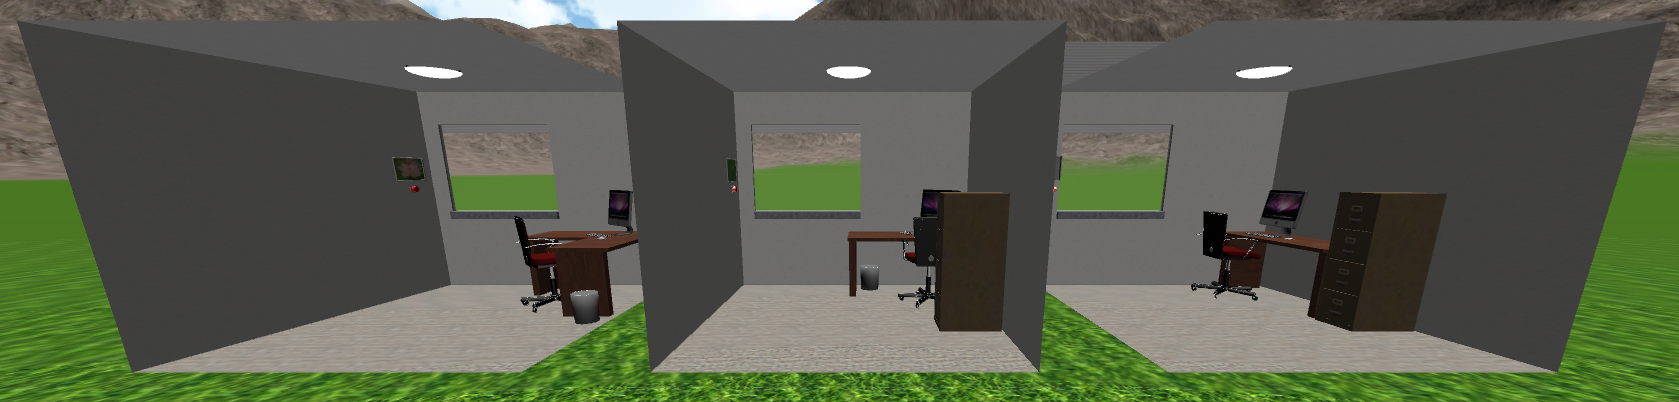
\includegraphics[width=\textwidth]{offices}
    \caption{De drie kantoren.}
    \label{fig:kantoren}
\end{figure}

Bij het betreden van de virtuele omgeving staat de proefpersoon aan het begin van
de gang, aan de rechtermuur zijn 4 deuren te zien, 80 cm breed met 80 cm er
tussen. Bij het betreden van het kantoor en het sluiten van de blinden wordt de 
hele gang naar achter verschoven zodat de deur nu aan de andere kant van de kamer 
staat zoals ge\"illustreerd in figuur \ref{fig:verandering}, na het verlaten van 
het kantoor staat de proefpersoon weer op de exacte locatie waar hij begonnen is.
Wegens de beweging van de gang wordt er hier de illusie gecre\"eerd dat men
verder in de gang staat dan eerst. De proefpersoon kan dan de deur van het 
kantoor sluiten om de volgende deur te openen. Dit geheel wordt drie keer 
herhaald. Om wat vari\"eteit te behouden zijn de drie kantoren, zoals 
ge\"illustreerd in figuur \ref{fig:kantoren}, lichtjes verschillend ontworpen. 
Enkel de knop om de blinden te sluiten en het fotokader er boven staat in ieder 
kantoor op dezelfde plaats.

\begin{figure}[h!]
    \centering
    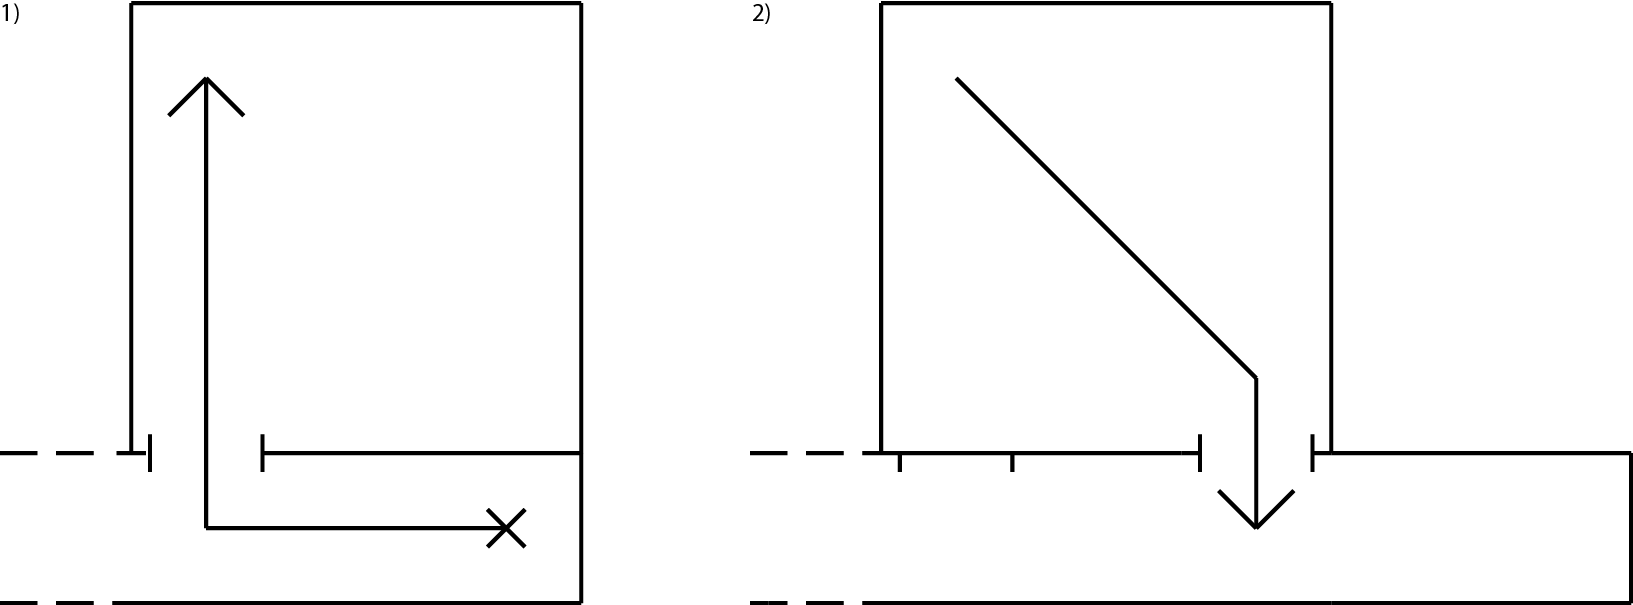
\includegraphics[width=\textwidth]{verandering}
    \caption{Verandering van de omgeving.}
    \label{fig:verandering}
\end{figure}

De beweging van de gang wordt teweeg gebracht door een transformatie in de
positie te laten gebeuren na het triggeren van de knop, wegens de implementatie
is de deur hier nooit voor in beeld. De vierde kamer dient enkel als markering 
van het einde, bij het betreden van deze kamer gaan de lichten langzaam uit.

Om een kleine hoeveelheid ruimte rondom de tracking area over te houden heb ik
een constante factor van 1.1 op de bewegingssnelheid toegepast daar dit klein 
genoeg is om onmerkbaar te zijn\cite{steinicke09}. Wegens de manier waarop dit 
systeem werkt is het onmogelijk om een grondplan te tekenen dat overeen komt met 
de realiteit, in figuur \ref{fig:plan} is te zien wat het beoogde mentale 
vloerplan is van de proefpersonen.

\begin{figure}[h!]
    \centering
    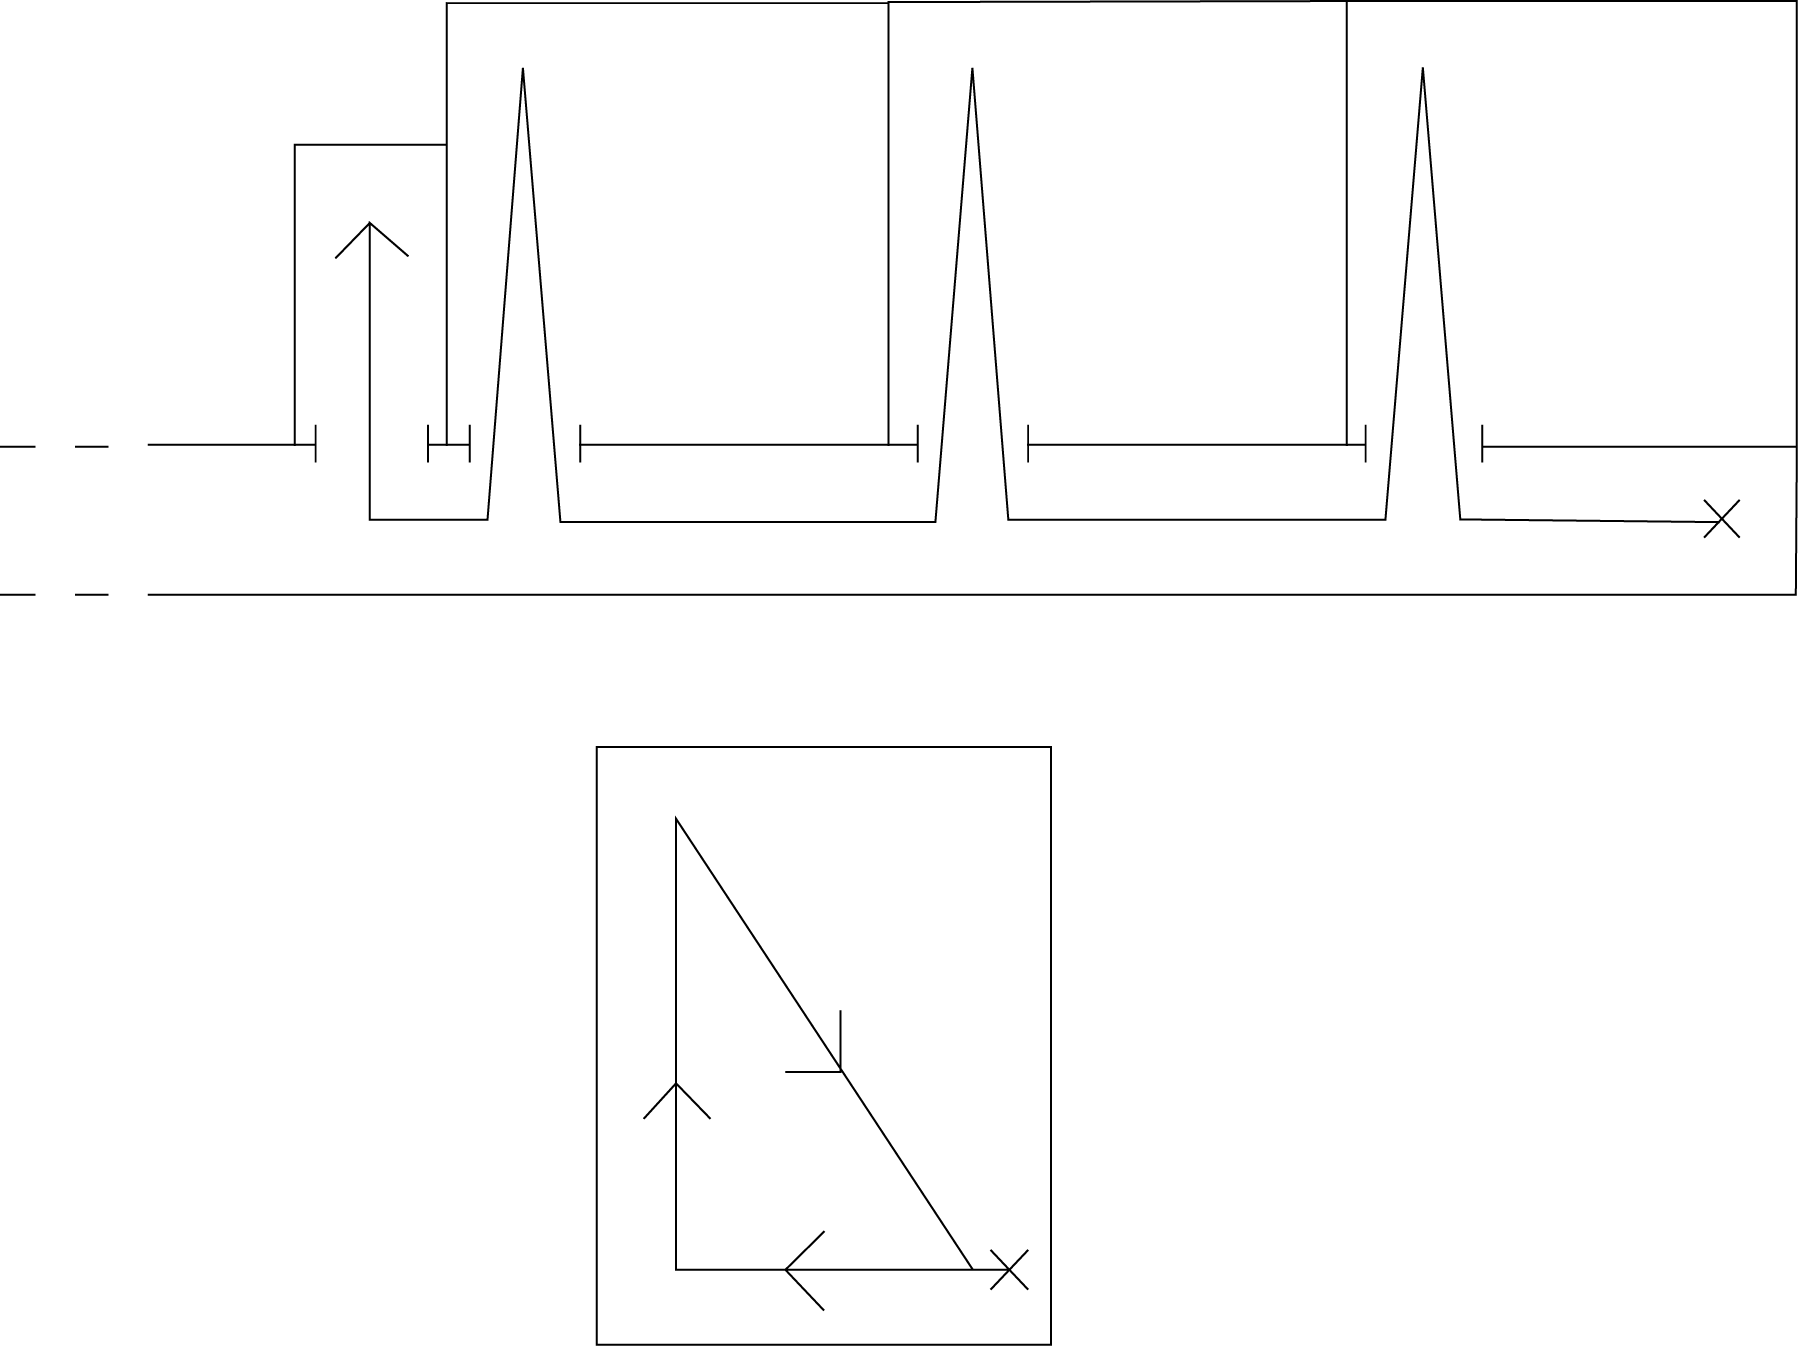
\includegraphics[width=\textwidth]{plan}
    \caption{Mentaal grondplan van de virtuele omgeving.}
    \label{fig:plan}
\end{figure}


\section{Implementatie}
\subsection{Engine}
Voor de implementatie van de virtuele omgeving heb ik er voor gekozen om met de
Unity engine te werken. Ik heb deze keuze gemaakt omdat de Unity engine relatief
eenvoudig is om mee te werken en mij meer tijd over laat om te werken aan de
benodigde algoritmen. Voor het ontwerp van de omgeving heb ik gebruik gemaakt 
van de Blender 3D editor, wegens eerdere ervaring met deze editor.

Ik beschrijf nu even kort de belangrijke details van mijn implementatie.


\subsubsection{Systeem state}
Voor de state van het systeem maak ik gebruik van stappen, er is op elk moment
slechts een object dat reageert op interactie. Wegens de volledig lineaire aard
van het systeem, en de relatief kleine hoeveelheid stappen is dit op de meest 
voor de hand liggende methode opgelost: Met een switch statement die de correcte
animaties dispatcht. Met wat onnodige details weggelaten ziet dit er zo uit:

\begin{minted}[mathescape, linenos, numbersep=5pt, frame=lines, framesep=2mm]{csharp}
// ...
private int _ctr = 1;
// ...

void Update() {
    // Decrement the delay between actions
    _timeout -= Time.deltaTime;

    // Check if a transition is requested, 
    // and that it is allowed by position, view and timeout
    if((Input.GetButtonDown("Activate")) && 
            _timeout <= 0f && 
            CanTriggerNextStep()) {
        // Reset the timeout
        _timeout = 1.5f;

        // Make the animation happen based on the active step
        switch(_ctr) {
        case 1: // Clicking button in room 1
            StartCoroutine(MoveHallway(0f, 0f, 1.6f));
            StartCoroutine(DescendBlinds());
            StartCoroutine(DepressButton());
            break;
        case 2: // Closing door of room 1
            StartCoroutine(RotateDoor(Door1));
            StartCoroutine(RespawnRoom(0.6f));
            StartCoroutine(RotateDoor(Door2, 0.6f, false));
            break;
        case 3: // Clicking button in room 2
            StartCoroutine(MoveHallway(0f, 0f, 1.6f));
            StartCoroutine(DescendBlinds());
            StartCoroutine(DepressButton());
            break;
        case 4: // Closing door of room 2
            StartCoroutine(RotateDoor(Door2));
            StartCoroutine(RespawnRoom(0.6f));
            StartCoroutine(RotateDoor(Door3, 0.6f, false));
            break;
        case 5: // Clicking button in room 3
            StartCoroutine(MoveHallway(0f, 0f, 1.6f));
            StartCoroutine(DescendBlinds());
            StartCoroutine(DepressButton());
            break;
        case 6: // Closing door of room 3
            StartCoroutine(RotateDoor(Door3));
            StartCoroutine(RespawnRoom(0.6f, 0f, -1f, 0f, -1.6f));
            StartCoroutine(RotateDoor(Door4, 0.6f, false));
            break;
        }

        // Increment the "step" of the process
        ++_ctr;
    }
}
\end{minted}


\subsubsection{Interactie}
Bij de activatie van deuren en knoppen wordt er eerst gekeken of de proefpersoon
zich op minder dan een meter afstand van het object bevind, en of hij het object
in beeld heeft. Als aan beide voorwaarden wordt voldaan wordt de animatie
geactiveerd.

Voor beide delen van deze check maak ik gebruik van de ingebouwde functionaliteit
van Unity. Lichtjes ingekort, ziet de code er zo uit:

\begin{minted}[mathescape, linenos, numbersep=5pt, frame=lines, framesep=2mm]{csharp}
bool CanTriggerNextStep(Transform object) {
    return InView(object) && Distance(object) <= 1f;
}

// Returns the distance on the XZ plane of our position to a point
float Distance(Vector3 pos) {
    Vector2 v1 = new Vector2(tracker.GetX(), tracker.GetY());
    Vector2 v2 = new Vector2(pos.x, pos.z);
    Debug.Log(Vector2.Distance(v1, v2));
    return Vector2.Distance(v1, v2);
}

// Is Vector3 in view
bool InView(Vector3 v) {
    v.y = Camera.main.transform.position.y;
    Vector3 vis = Camera.main.WorldToViewportPoint(v);
    if((vis.x < 0 || vis.x > 1) || vis.z <= 0) {
        return false;
    }
    return true;
}
\end{minted}


\subsubsection{Animatie}
Voor de animaties maak ik gebruik van sferische lineaire interpolatie tussen de
begin- en de eindpositie van de te animeren objecten.

Sferische lineaire interpolatie wordt standaard door Unity meegeleverd. Volgende
stukjes code tonen de implementatie van respectievelijk het laten dalen van de
blinden, het indrukken van de knoppen, en het sluiten van de deuren.

\begin{minted}[mathescape, linenos, numbersep=5pt, frame=lines, framesep=2mm]{csharp}
// Play the animation for closing the blinds
IEnumerator DescendBlinds(float delay = 0f) {
    yield return new WaitForSeconds(delay);
    Vector3 begin = _blinds.transform.position;
    Vector3 end = begin - new Vector3(0f, 0.995f, 0f);

    for(float i = 0f; i < 1.5f; i += Time.deltaTime) {
        _blinds.transform.position = Vector3.Slerp(begin, end, 
                i / 1.5f);
        yield return true;
    }

    _blinds.transform.position = end;
    yield return true;
}

// Play the animation for pressing the button
IEnumerator DepressButton(float delay = 0f, 
        bool isRotated = false) {
    yield return new WaitForSeconds(delay);
    Vector3 begin = _button.transform.position;
    Vector3 end = begin + (isRotated ? new Vector3(0.03f, 0f, 0f) : 
            new Vector3(0f, 0f, -0.03f));

    for(float i = 0f; i < 0.25f; i += Time.deltaTime) {
        _button.transform.position = Vector3.Slerp(begin, end, 
                i / 0.25f);
        yield return true;
    }

    _button.transform.position = end;
    yield return true;
}

// Open or close a door, meaning a 90 degree rotation in a 
// certain direction
IEnumerator RotateDoor(GameObject door, float delay = 0f, 
        bool close = true) {
    yield return new WaitForSeconds(delay);

    float angle = door.transform.rotation.eulerAngles.y;
    float goal = close ? angle - 90 : angle + 90;
    Quaternion end = Quaternion.AngleAxis(goal, Vector3.up);
    Quaternion begin = door.transform.rotation;

    for(float i = 0f; i < 0.5f; i += Time.deltaTime) {
        door.transform.rotation = Quaternion.Slerp(begin, end, 
                i / 0.5f);
        yield return true;
    }

    door.transform.rotation = end;
    yield return true;
}
\end{minted}

Voor de ``animatie'' van de beweging van de gang wordt er helemaal geen animatie
gedaan, omdat deze niet in het zicht van de proefpersoon is. Daar de deuren in
het object van de gang verwerkt zitten, is deze beweging de effectieve
implementatie van change blindness in deze virtuele omgeving.

\begin{minted}[mathescape, linenos, numbersep=5pt, frame=lines, framesep=2mm]{csharp}
// Move the hallway 1.6m back.
IEnumerator MoveHallway(float x, float y, float z, 
        float delay = 0) {
    yield return new WaitForSeconds(delay);
    Hallway.transform.Translate(x, y, z);
    yield return true;
}
\end{minted}

\subsection{Tracking}
Voor integratie met het trackingsysteem heb ik gebruik gemaakt van de gratis
editie van de MiddleVR middleware\cite{middlevr}. Deze maakt het mogelijk om via 
het VRPN protocol te communiceren met de tracking server.

MiddleVR geeft ook toegang tot ``virtual trackers'' waarmee men de data van een
tracker kan transformeren. Het resultaat hiervan is dat ik de pitch en de roll
van de HMD heb kunnen gebruiken, en de yaw van het camera tracking systeem. Dit
omdat de HMD een kleine hoeveelheid ``yaw drift'' heeft, en dit zou kunnen zorgen
voor botsingen met de fysieke omgeving.

Ik heb dit systeem ook gebruikt om de trillingen in de gerapporteerde yaw van het
trackingsysteem te verminderen door een gemiddelde van twee metingen te 
gebruiken. Daar de \emph{framerate} van het systeem voldoende is, heeft dit bijna 
geen effect op de latency van de bewegingen (effectief een latency van 16 ms bij
een framerate van 60 Hz). In de praktijk werkt dit door te werken met het 
gemiddelde van de vorige meting en de nieuwe meting in plaats van met de rauwe 
meting.

\begin{minted}[mathescape, linenos, numbersep=5pt, frame=lines, framesep=2mm]{csharp}
private float getModifiedYaw() {
    // Get yaw from optitrack tracker.
    float a = optiTrack.GetYaw() - yawZeroOpti;
    a = normAngle(a);

    // If not first frame, take avg of last 2 measurements.
    if(!firstFrame) {
        if(Mathf.Abs(a - prevYaw) > 180.0f) {
            if(a > prevYaw) {
                prevYaw += 360.0f;
            } else {
                a += 360.0f;
            }
        }
        a = (a + prevYaw) / 2.0f;
    }
    a = normAngle(a);
    prevYaw = a;

    return a - 180.0f;
}

private float normAngle(float a) {
    while(a < 0) {
        a += 360;
    }

    while(a >= 360) {
        a -= 360;
    }

    return a;
}
\end{minted}

Ik heb hier uitdrukkelijk geen gebruik gemaakt van een Kalman filter wegens de
precisie van het OptiTrack systeem tot op minder dan een millimeter. Hierdoor
is mijn techniek ruim voldoende om de zeer kleine hoeveelheid jitter op te
vangen.

Aan de serverkant heb ik gebruik gemaakt van de OptiTrack:Motive software om de
VRPN data te broadcasten.


\subsection{Hardware}
Om een vloeiende werking te verzekeren werd de virtuele omgeving gedraaid op een
Apple MacBook Pro met een 2,5 GHz Intel Core i5 processor, 8 GB 1333 MHz DDR3 RAM
geheugen en een Intel HD Graphics 4000 GPU. Het beeld werd getoond op een Oculus 
Rift (Devkit 1) aan 60 fps voor beide ogen. Deze HMD heeft een diagonale FoV van 
110\textdegree{} en vult hierdoor bijna het hele zicht van de proefpersonen voor 
een maximale immersie.

Tracking van positie en rotatie in 3 assen werd gedaan door een 6 camera
OptiTrack systeem rondom een 3 m x 4 m omgeving. Om gebruikersinvoer te voorzien 
heb ik gewoon een bluetooth muis gebruikt, zodat de proefpersoon op eender welke 
knop kon klikken om het object voor hem te activeren.